
\subsection{Photon Detector UV-Light Monitoring System}
\label{sec_pd_calib}

\fixme{Anne removed all commented text from previous version; it is still available in the repository if needed. 8/18}

% NOT NEEDED  	As already described, the baseline for the scintillation photon detectors assumes deployment of light collection paddles to reduce the required costly photo-cathode area. Several photon detector designs are presently being developed and have been tested in small dewars or in recent DUNE's 35 ton prototype. Since each of these new elements has not yet been tested in realistically large-scale TPC, the protoDUNE LArTPC prototype is being constructed to provide essential design validation. 
\fixme{next pgraph should be up higher}	The current DUNE Far Detector designs are anticipated to have sufficient sensitivity to provide event timing information for atmospheric neutrino and proton decay channels, but sufficient efficiency down to the 5 MeV neutrino energy level desired by the supernova program has to be demonstrated in future designs.

%In the absence of precise physics requirements for the photon detector system and in order to support R\&D activities on the photon detector development it was decided that the photon detector should provide a time stamp to determine the time of occurrence of an event (so called "time zero") with an accuracy much better than 30 ns.	Items relevant to the photon detector calibration are the fast and slow components of the light, photon propagation including scattering and reflections, impact of N$_2$, E-field strength, as well as the energy range of interest. A calibration system that addresses the issues listed above has to be both comprehensive and cost-effective, and has to be tied to the overall calibration system for protoDUNE, that includes both charge and scintillation light calibration techniques. In addition, there is a need to evaluate relative efficiencies of multiple photon-detector units and monitor response and stability of the system as a function of time.An UV-light based calibration system that will serve to monitor the relative performance and time resolution of the system has been designed and is described here.The system will consist of a set of UV LEDs as light sources in VUV wave-length range, coupled to quartz fibers, to transmit light from outside the detector volume to desired locations at the CPA within a TPC.Light sources located at CPA surface will uniformly illuminate APA area with photon-detector sensitive elements. Therefore we will equip the protoDUNE detector with light sources located and fired externally, with fibers running into the cryostat, to diffusers that will emit light from the CPA to the APA. For the protoDUNE cryostat at the surface at CERN the UV-light system will be complementary to cosmic ray muon tracks and Michel electrons as means of calibration. In terms of light sources the measurements will be performed with an UV (245-280) light source. The UV light essentially mimics physics, although at a different wave-length starting from the wavelength shifter conversion, light guide propagation, photo-sensor detection and the front-end electronics readout.

\fixme{next pgraph should be up higher} In the absence of precise physics requirements for the PDS and in order to support R\&D activities on the PD development it was decided that the PDS should provide a time stamp to determine the time of occurrence of an event (so called \textit{time zero}) with an accuracy much better than 30~ns.

		Items relevant to the PDS calibration are the fast and slow components of the light, photon propagation including scattering and reflections, impact of N$_2$, E-field strength, 
and the energy range of interest. A calibration system that addresses these issues has to be both comprehensive and cost-effective, and has to be tied to the overall 
calibration system for ProtoDUNE-SP, which includes both charge and scintillation light calibration techniques. 
In addition, there is a need to evaluate relative efficiencies of multiple PD units and monitor response and stability of the system as a function of time.

A UV-light-based calibration system that will serve to monitor the relative performance and time resolution of the system has been designed. % and is described here.
The system will consist of a set of UV LEDs as light sources in the VUV wavelength range, coupled to quartz fibers, to transmit light from outside the detector volume to desired locations at the CPA within the TPC.
\fixme{Additional?} Light sources located at the CPA surface \fixme{these aren't the other ends of the fibers fed into diffusers?} will uniformly illuminate the APA area with photon-detector sensitive elements. \fixme{photon sensitive elements?} Therefore we will equip the ProtoDUNE-SP detector with light sources located and fired externally, 
with fibers running into the cryostat, to diffusers that will emit light from the CPA to the APA. \fixme{put `diffusers' in other sentence and get rid of previous sentence.}  For the ProtoDUNE-SP cryostat at the surface at CERN, the UV light system \fixme{VUV?} will be complementary to cosmic ray muon 
tracks and Michel electrons as means of calibration. In terms of light sources the measurements will be performed with an UV (245-280) light source. The UV light essentially mimics physics, although at a different 
wavelength starting from the wavelength-shifter conversion, light guide propagation, photo-sensor detection and the front-end electronics readout.

\fixme{clarify a few things: are there two light sources, one external and another one internal?  If one only, is it near UV (245-280 nm) or VUV (under 200nm)?}
	
		
				The external light-flasher calibration system is designed under following assumptions:\fixme{mention the flasher higher up. Also, these sound like requirements, not assumptions }
				
\begin{itemize}
\item Simple to implement (no active components within PD/APA, such as LEDs or fibers mounted within APA).
\item Uniformly illuminates APA surface with the light diffused from CPA locations.
\item Has a potential to be adapted for deployment in a large Far Detector in the future
\end{itemize}

	In terms of technical requirements the system needs to:
\begin{itemize}
\item provide light levels down to a single p.e. at individual photon-detector channels,
\item provide higher light levels to test linearity of the PDS,
\item provide variable pulse width to test the time resolution of the photon detector response, and
\item uniformly illuminate the APA area of the detector for relative monitoring of the PDS channels
\end{itemize}

Figure~\ref{fig:fig-c-1} illustrates the system design schematically. The system consists of a 1U rack mount Light Calibration Module (LCM) sitting outside the cryostat. The LCM generates light pulses that propagate through a quartz fiber-optic cable to diffusers at the CPA to distribute the light uniformly across the photon detectors mounted within the APA.  ProtoDUNE-SP will have five light 
diffusers on the CPA plane: one in the center and four diffusers close to the CPA corners, as illustrated in Figure~\ref{fig:fig-c-2}. 
%
 \begin{cdrfigure}[UV-light monitoring system]{fig:fig-c-1}{Concept of the UV-light monitoring system for the photon detector in liquid argon.}
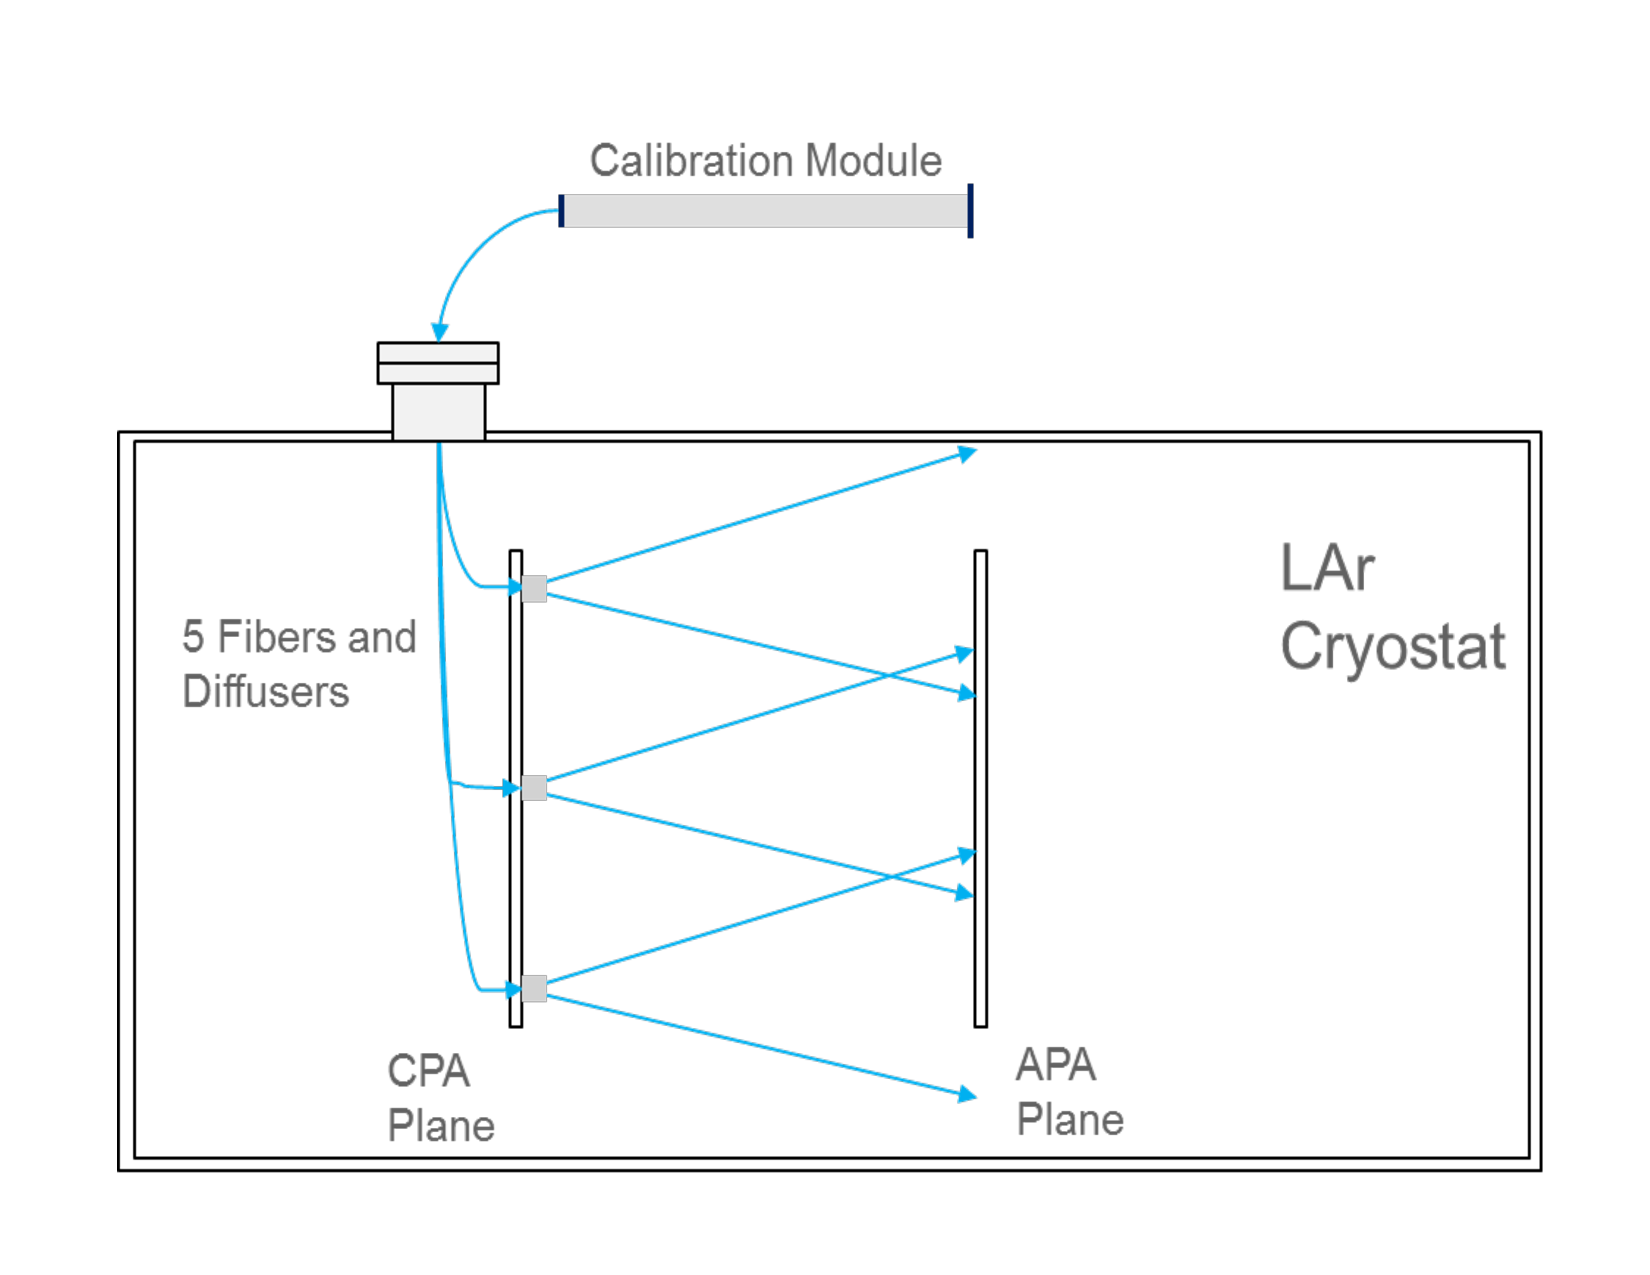
\includegraphics[angle=0,width=10cm,height=7cm]{calPD_concept-from-35ton.pdf}
\end{cdrfigure}
%
%
\begin{cdrfigure}[Deployment of PDS UV-light monitoring system]{fig-c-2}{The diffuse light is emitted from diffusers (top and bottom left figure) mounted at five CPA locations, indicated by arrows (right figure). 
The UV light from the light calibration system to diffusers is transported through quartz fiber.}
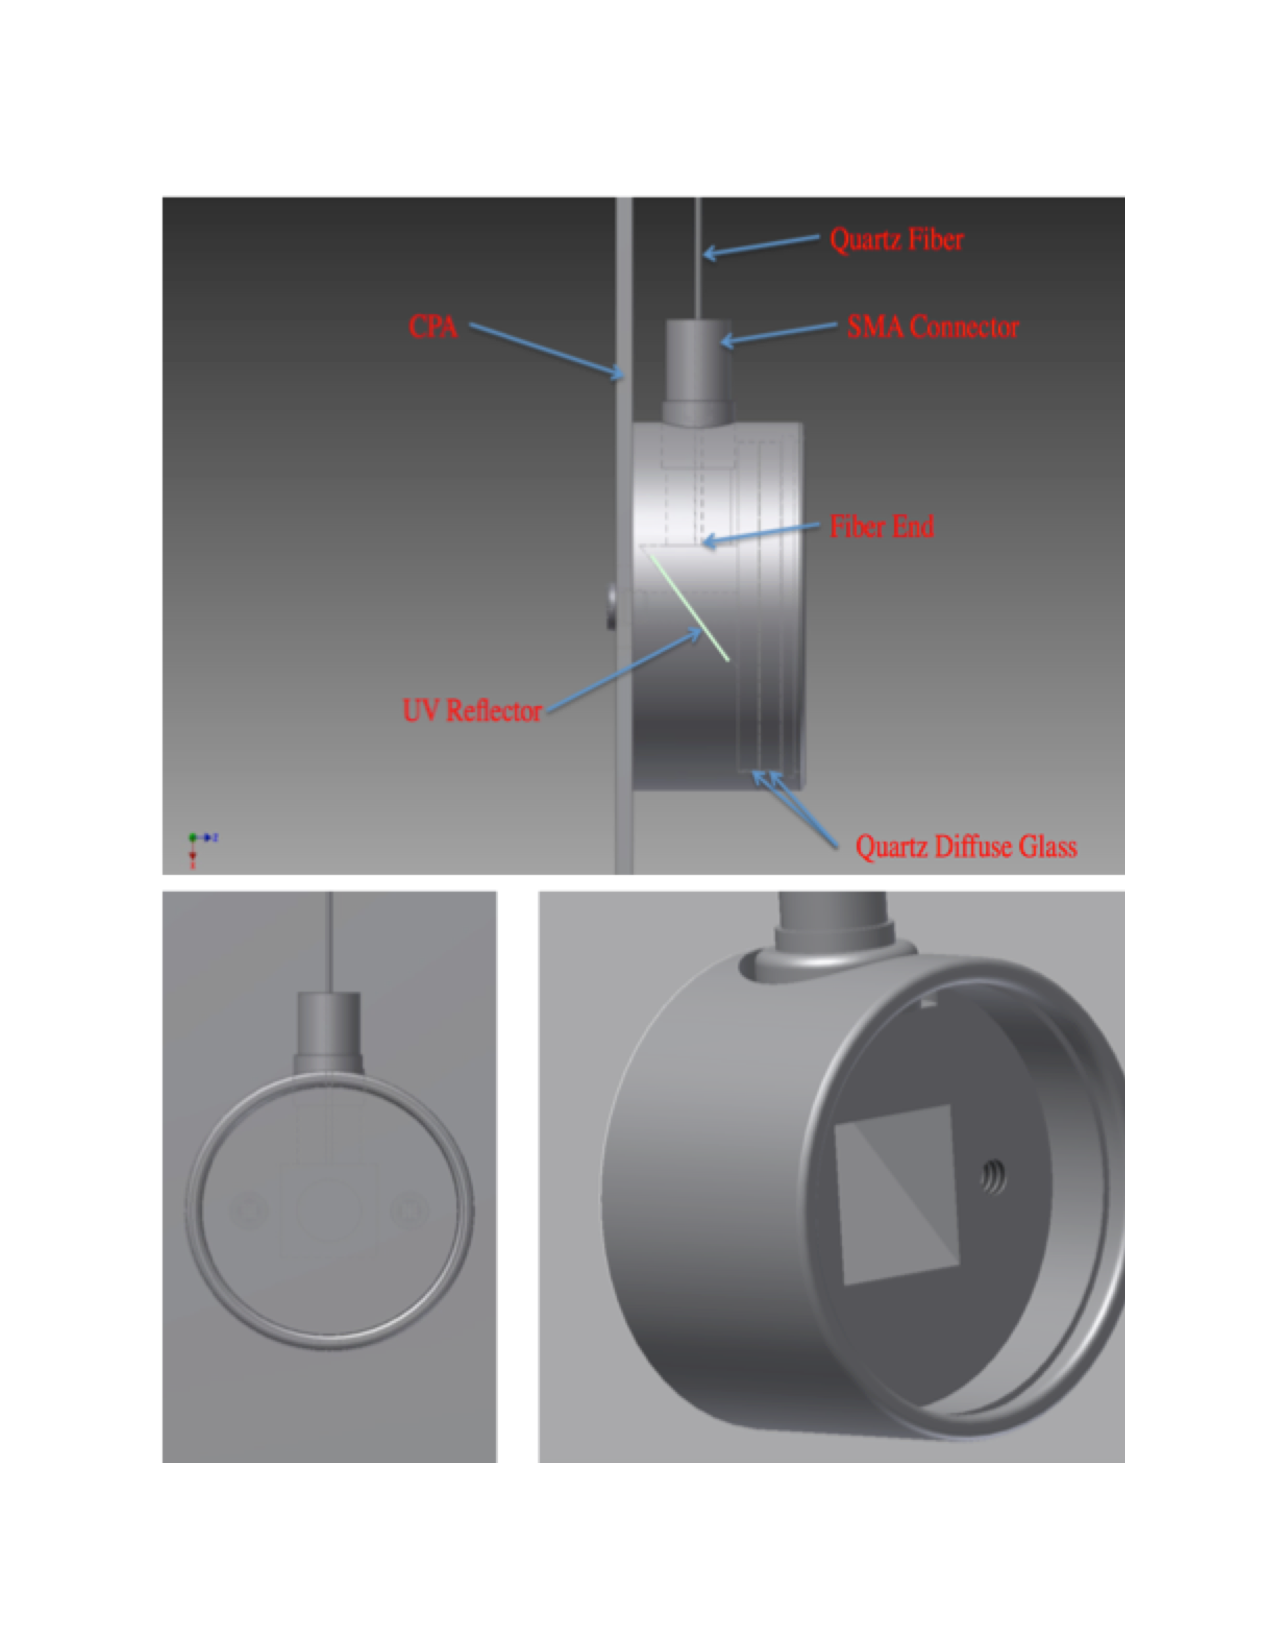
\includegraphics[angle=0,width=0.4\textwidth]{calPD_Calibration_diffuser_system_protoDUNE_slide_left_half.pdf}
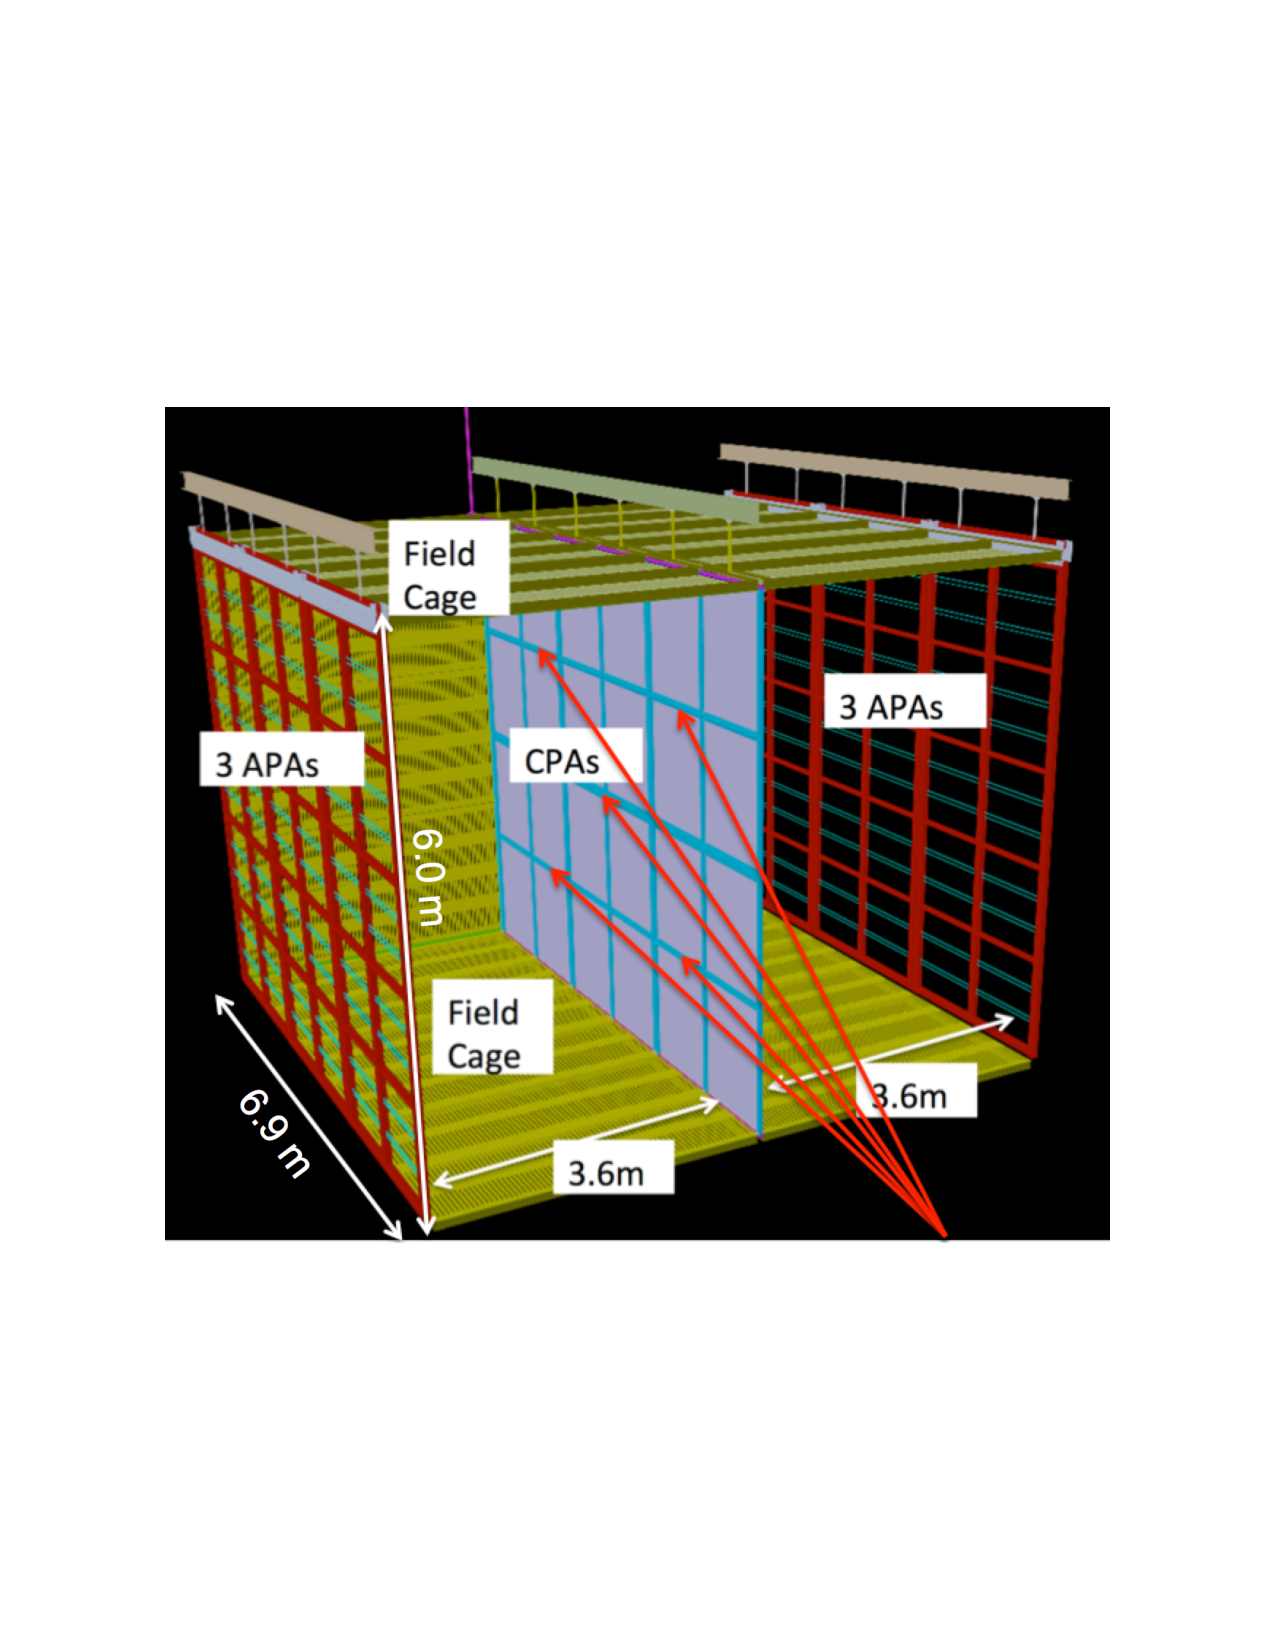
\includegraphics[angle=0,width=0.55\textwidth]{calPD_Calib_diffuser_locations_protoDUNE.pdf}
\end{cdrfigure}

\fixme{left hand figure's text is way too small}
%
%
For the 280-nm light \fixme{is this what you're calling VUV? Or just UV? Please use consistent terminology throughout} a simulation of the designed diffuse light calibration system has been performed using TracePro, a generalized 3D light ray-tracing program with the ability 
to include bulk optical properties such as absorption, fluorescence, and birefringence in addition to surface properties such as scattering and reflection. 
As an example, Figure~\ref{fig:fig-c-4} shows simulated light distributions at an APA surface for the cases of the VUV light emitted by either the central diffuser only (left figure), 
or by the outer four diffusers simultaneously (right figure). 

%
 \begin{cdrfigure}[UV-light monitoring illumination calculation]{fig:fig-c-4}{Simulated light distributions of at the APA location for the cases of the VUV light emitted by either the central diffuser only (left figure), or by outer four diffusers simultaneously (right figure).
The simulation estimate has been obtained for 35-ton detector and scaled by to 3.6 m CPA - APA distance at ProtoDUNE-SP.}
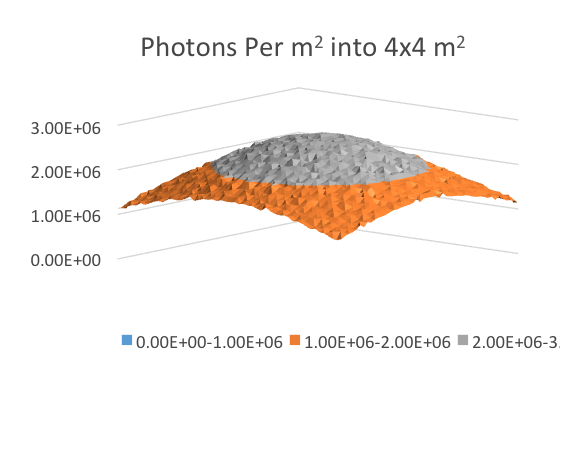
\includegraphics[angle=0,width=6.5cm,height=6cm]{calPD_4mx4m-area-3point6m-away-quantified.png}
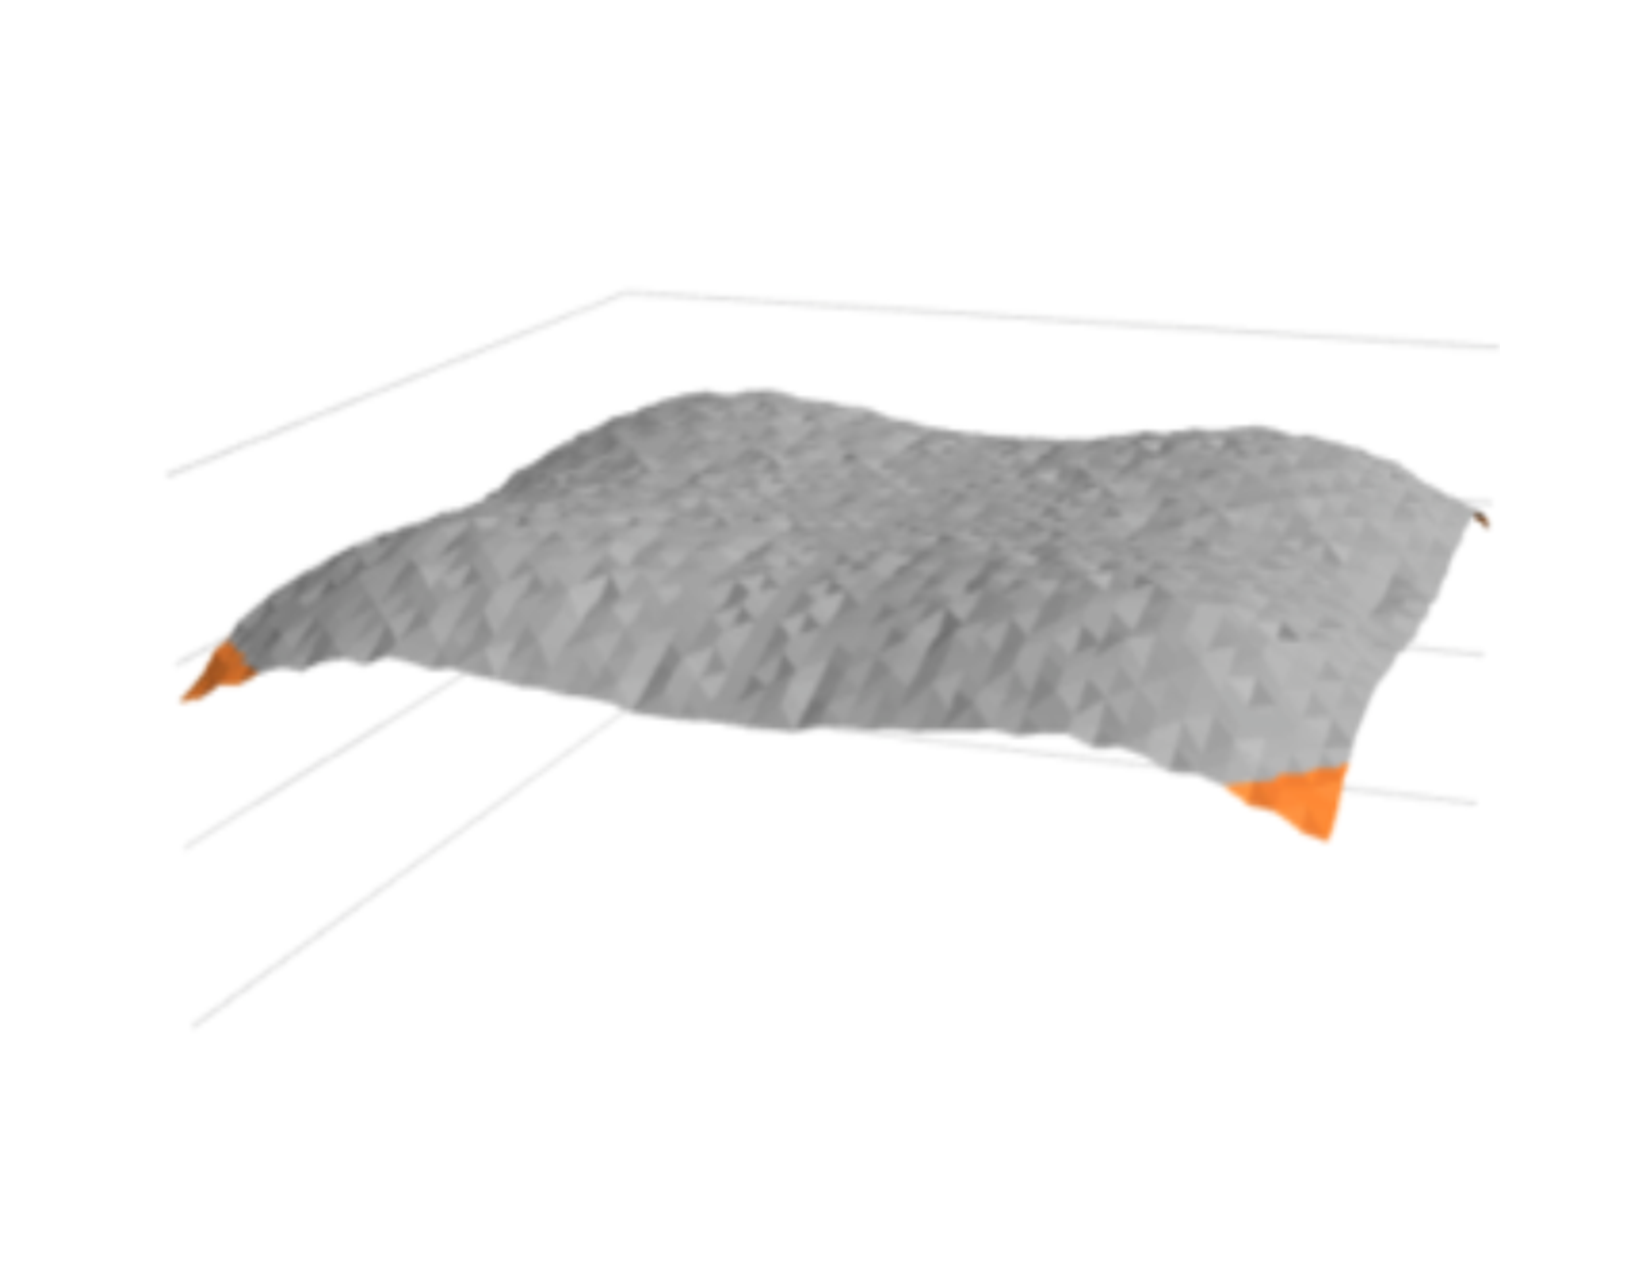
\includegraphics[angle=0,width=6.5cm,height=6cm]{calPD_figR.pdf}
\end{cdrfigure}
%

The LCM as well as the full prototype of the light calibration system system has been built, tested and successfully operated with 35-ton LArTPC at Fermilab. The LCM is shown in Figure~\ref{fig:fig-c-3}. 

The ANL photon calibration module \fixme{from Argonne? Spell out at first reference. And is this a different one?} combines the logic developed with the photon-detector readout electronics (so-called "SSP") unit.  
\fixme{combines logic with readout elec?  or combines the logic `developed with readout elec' and something else?}
For this design an SSP board was essentially repackaged into a deeper rack mount 
chassis \fixme{deeper than what?} that accommodates a new internal LED Pulser Module (LPM) and an additional bulk power supply. The LPM utilizes five digital outputs to control the LPM pulse and its duration.  
These outputs are derived from the charge injection control logic within the SSP's FPGA.  The even-channel SiPM bias DACs \fixme{dig to analog converter?} are used to control the LPM pulse amplitude.  
The adjacent odd channels are used to read out a reference photodiode used for pulse-by-pulse monitoring of the LED light output.  The output of the monitoring diode may be used to normalize 
the response of the SiPMs in the detector to the calibration pulse.

%
 \begin{cdrfigure}[]{fig:fig-c-3}{Photon detector light calibration module (LCM) front (left) and back (right) ends.}
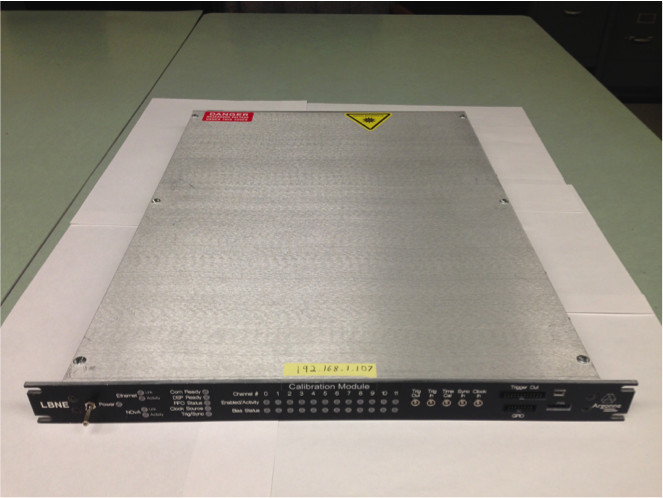
\includegraphics[angle=0,width=7cm,height=4.5cm]{calPD_LCM_front.png}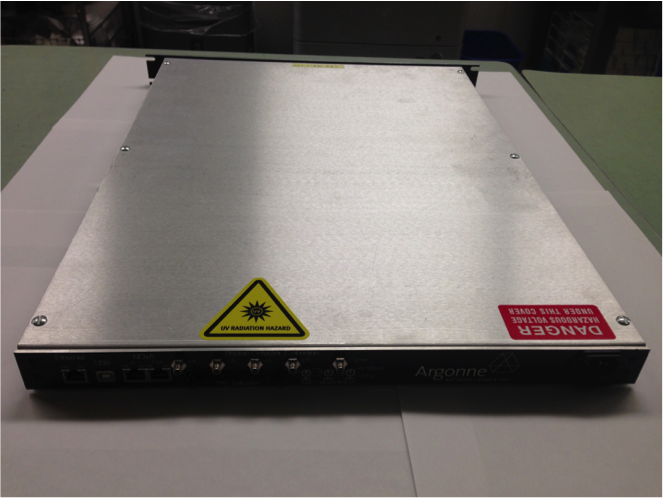
\includegraphics[angle=0,width=7cm,height=4.5cm]{calPD_LCM_back.png}
\end{cdrfigure}


%A prototype of this light calibration monitoring system has been designed, tested, installed, integrated, and operated with the 35-ton DUNE prototype detector.
The data from the 35-ton test is currently being analyzed. %As en example of the system tests in former 35-ton detector in 
Figure~\ref{fig:fig-wf} shows SSP waveforms collected as a response to the light calibration system % described here.
%This data has been collected 
in liquid argon, with the TPC powered-on, and at the nominal value of drift high-voltage. \fixme{what is the value?} 
%at 35-ton detector. 
The length of optical fiber cables used %with the 35-ton detector 
was $\sim$22 m total, including external fibers (7 m), and fiber feed-through and internal fibers (15 m).

%
 \begin{cdrfigure}[Detected UV-light monitoring system light pulses]{fig:fig-wf}{Photon detector light calibration pulses detected by readout electronics. Recorded waveforms have range from few photo-electrons (left figure), to tens of photo-electrons (middle figure), to hundreds of photo-electrons (right figure).}
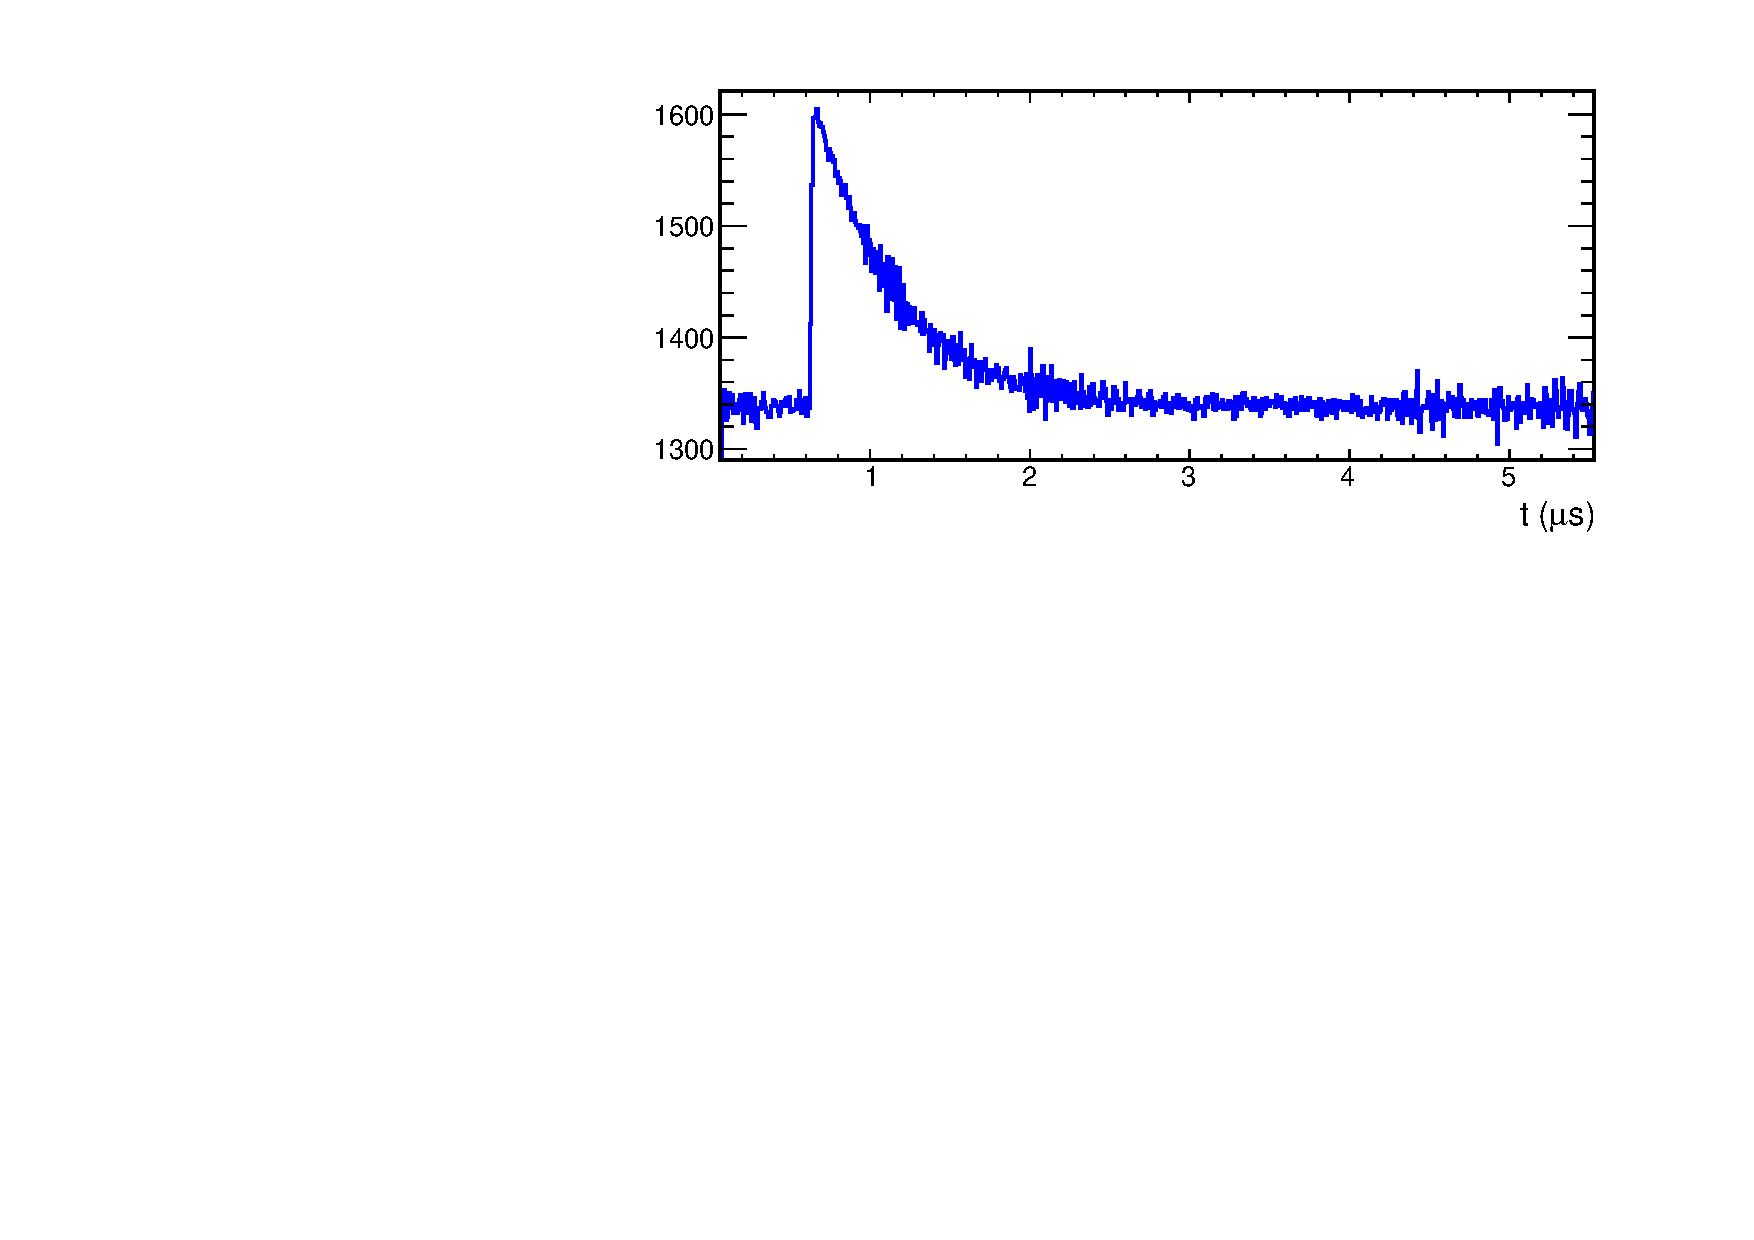
\includegraphics[angle=0,width=5cm,height=4cm]{calPD_example_ch21_run18573.pdf}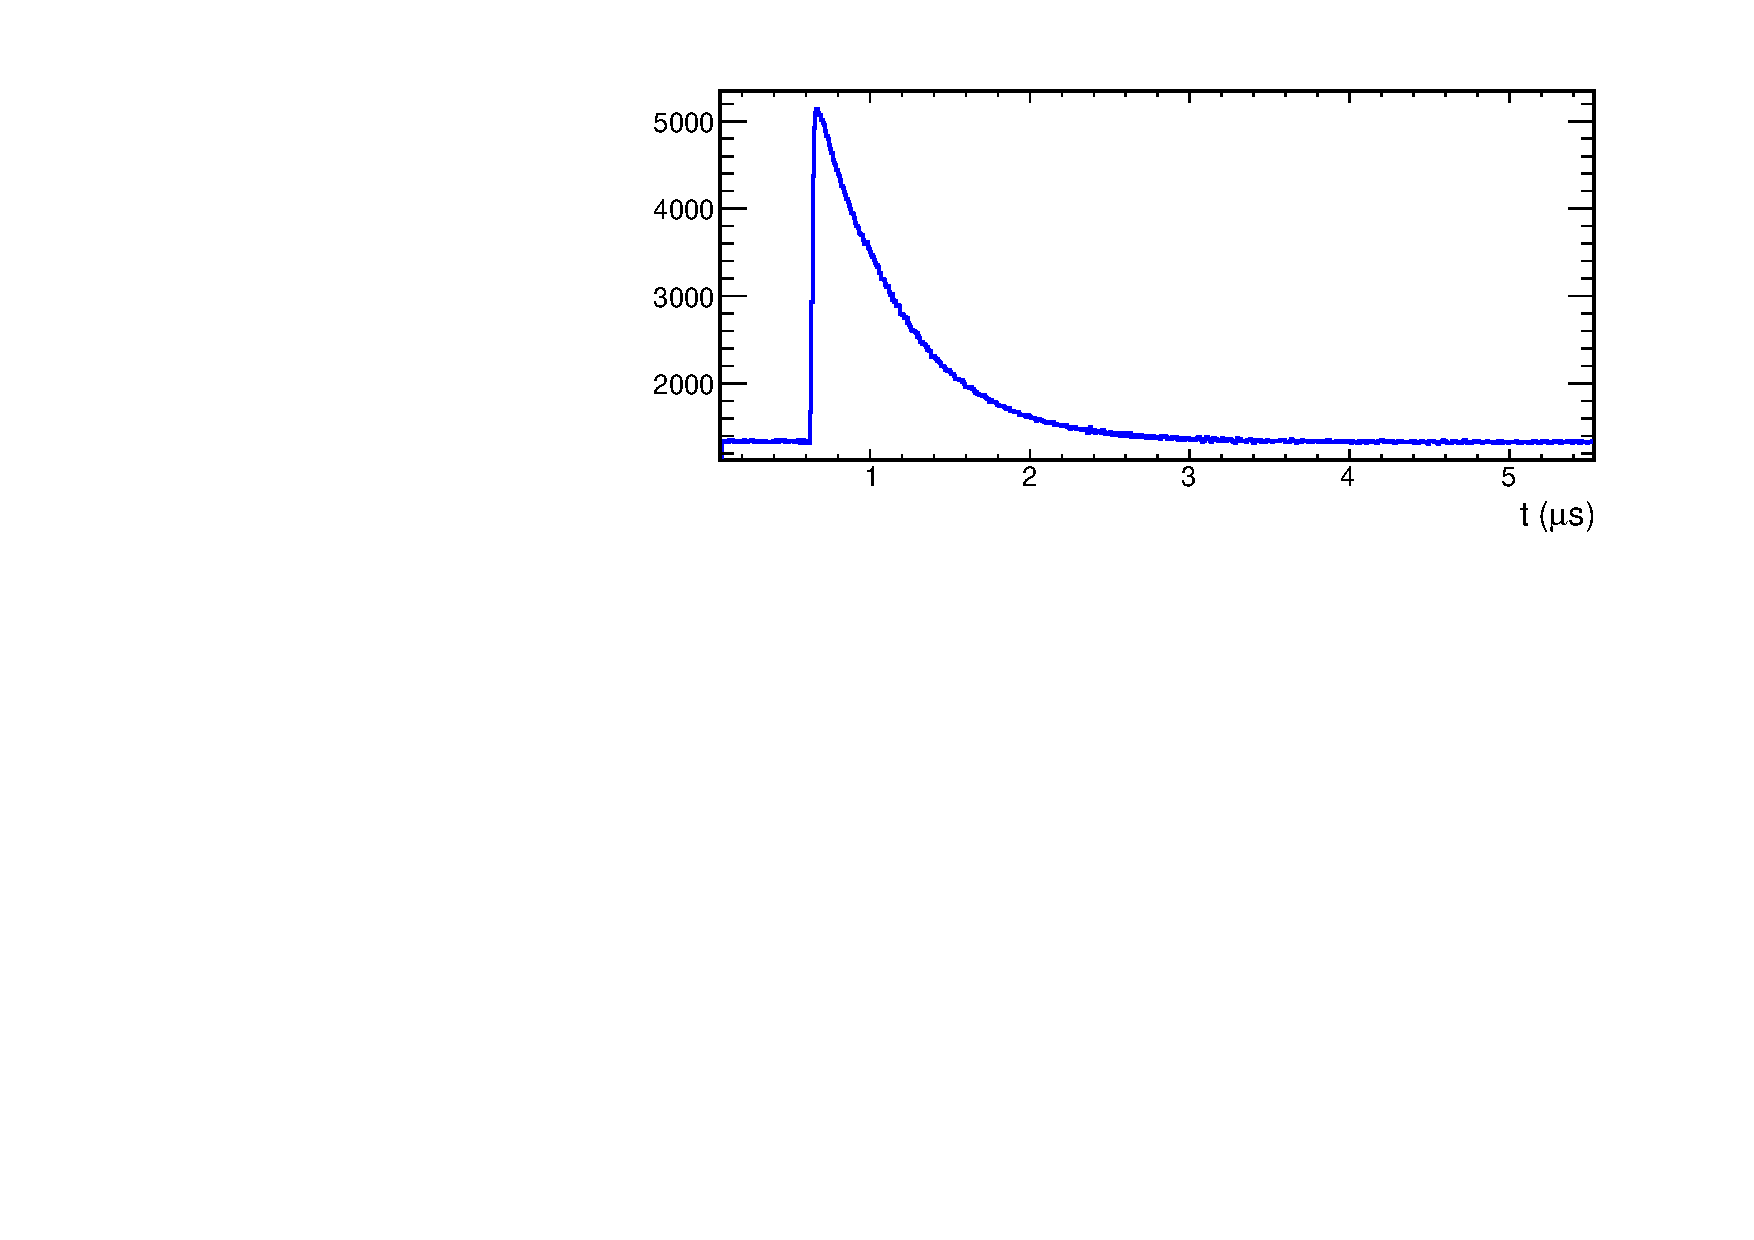
\includegraphics[angle=0,width=5cm,height=4cm]{calPD_example_ch21_run18574.pdf}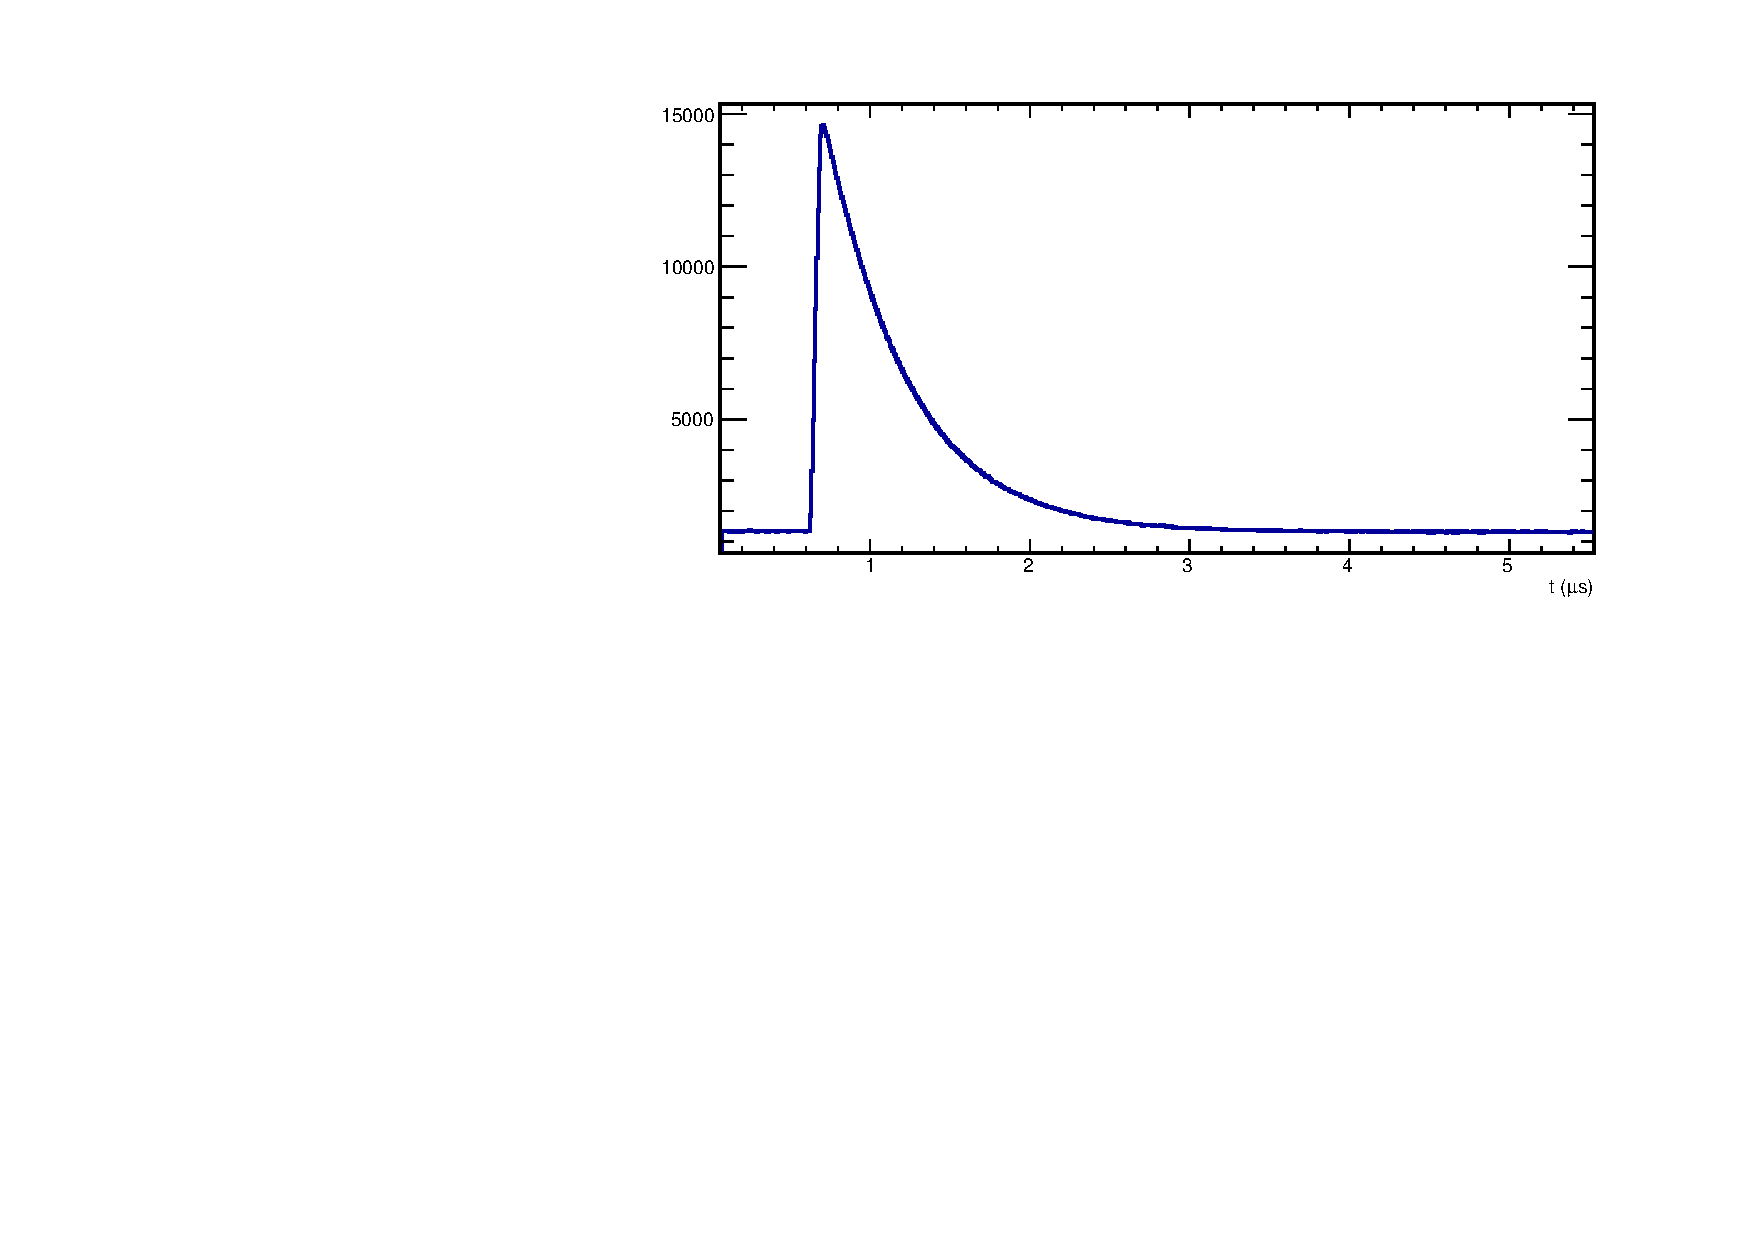
\includegraphics[angle=0,width=5cm,height=4cm]{calPD_example_ch21_run18572.pdf}
\end{cdrfigure}
%
In the DUNE prototypes (e.g., the ProtoDUNE-SP) and in future DUNE far detector modules it will be important to %check if 
verify the proper functioning of photon-detector components %are functioning properly 
at various stages of the detector operation. 
Periodic light-source deployments will monitor the system's stability as a function of time. A change in relative difference of UV light responses would point towards potential wavelength shifter instability, 
or changes in SiPM gain and/or collection efficiencies. %Much of the same monitoring is expected to be doable with cosmic rays in the ProtoDUNE-SP (at surface), with 
Periodic LED calibration runs will be complemented 
with cosmic-ray data tracked by an external hodoscope. 
%With the ProtoDUNE-SP detector one could use a well-defined muon trajectory defined by the hodoscope geometry and monitor the number of PEs per MeV of deposited charge. 
A well-defined muon trajectory defined by the hodoscope geometry could be used to monitor the number of p.e.'s per MeV of deposited charge, which in turn 
%The number of p.e.'s per photon-detector channel from the well defined muon track 
could be used as a calibration constant. This technique will likely be unusable 
%However, 
for the deep underground DUNE detectors since the cosmic ray flux may be inadequate. % for timely monitoring of the photon detectors.
	Two sets of calibration runs are planned for the ProtoDUNE-SP detector: 
\begin{enumerate}
\item Calibration runs with four outer diffusers run simultaneously, in order to
   \begin{itemize}
   \item measure response of PDS channels in multi-p.e. range and get integrated number of event samples for each channel (for maximum light output);
   \item test  the dynamic range from 1 p.e. to maximum number of p.e.'s; and
   \item repeat runs periodically to trace any changes in channel response.
    \end{itemize}
\item Runs with central diffuser only, in order to
   \begin{itemize}
   \item perform initial calibration runs that will reveal malfunctioning channels, if any;
   \item perform timing measurements with the 10--50-ns pulses; and
    \item verify time resolution of the PDS.
   \end{itemize}
\end{enumerate}

The controlled source of light %described here 
in this calibration system will be used to perform a relative $t_0$ calibration, \fixme{relative to what?} where the $t_0$ could be absolutely calibrated \fixme{calibrated absolutely or known absolutely?} with the use of the cosmic 
ray triggers available with ProtoDUNE-SP detector. 
Effects that contribute to a finite time resolution and relative time offset of photon-detector channels include scintillation time constants, 
photon conversion with wavelength shifter, photon propagation through photon-detector paddle, SiPM jitter, and FEE resolution. Most of these effects are constant and can be individually 
measured on the bench, so the LED flasher system will monitor overall stability of the photon detector.
\fixme{This last pgraph needs some work}
